%%%%%%%%%%%%%%%%%%%%%%%%%%%%%%%%%%%%%%%%%%%%%%%%%%%%%%%
% Please note that whilst this template provides a 
% preview of the typeset manuscript for submission, it 
% will not necessarily be the final publication layout.
%
% letterpaper/a4paper: US/UK paper size toggle
% num-refs/alpha-refs: numeric/author-year citation and bibliography toggle

%\documentclass[letterpaper]{aejstyles}
\documentclass[a4paper,alpha-refs]{eSpectra}

%%% Journal toggle; only specific options recognised.
\journal{aej}

\usepackage{graphicx}
\usepackage{siunitx}
\usepackage[spanish]{babel}             % Spanish for default (Abstract. References, Appendix, tables, and figures names).


 \usepackage{comment} 

 
%\usepackage[left]{lineno}
%\linenumbers

%%% Flushend: You can add this package to automatically balance the final page, but if things go awry (e.g. section contents appearing out-of-order or entire blocks or paragraphs are coloured), remove it!
% \usepackage{flushend}

\title{Título del artículo}

%%% Use the \authfn to add symbols for additional footnotes, if any. 1 is reserved for correspondence emails; then continuing with 2 etc for contributions.
\author[1,\authfn{1},]{Nombre y Apellido}
\author[2,\authfn{2}]{Nombre y Apellido}
\author[3]{Nombre y Apellido}

\affil[1]{Afiliación}
\affil[2]{Afiliación}

%%% Author Notes
\authnote{\authfn{1}Estudiante de Maestría en Ciencias - Astronomía (correo electrónico)}
\authnote{\authfn{2}Estudiante de Física (correo electrónico)}

%%% Paper category: Other categories include: Research Article, Review, News, Announcements, Interviews, Opinion, Resources & Activities, Book Review, Correspondences, Best practice,
\papercat{Artículo Científico}

%%% "Short" author for running page header
\runningauthor{First et al.}

%%% Should only be set by an editor
\jvolume{1}
\jnumber{1}
\jyear{2023}
\begin{document}
\begin{frontmatter}
\maketitle
\begin{abstract}
Escribir un resumen del trabajo que no supoere las 250 palabras.
\end{abstract}

\begin{keywords}
Colocar un máximo de 5 palabras claves, separadas por ";". 
\end{keywords}
\end{frontmatter}

\section{Introducción}

Introducción del artículo.

\section{Métodos}

Descripción de los métodos utilizados.

\subsection{Ecuaciones}

Ejemplo de ecuación:

\begin{equation}
    E = mc^2
\end{equation}

\subsection{Tablas}

Ejemplo de tabla:

\begin{table}[htb]
    \centering
    \caption{Ejemplo de tabla}
    \label{tab:ejemplo}
    \begin{tabular}{|c|c|c|}
        \hline
        Col 1 & Col 2 & Col 3 \\
        \hline
        1 & 2 & 3 \\
        4 & 5 & 6 \\
        7 & 8 & 9 \\
        \hline
    \end{tabular}
\end{table}

\subsection{Figuras}

Ejemplo de figura:

\begin{figure}[htb]
    \centering
        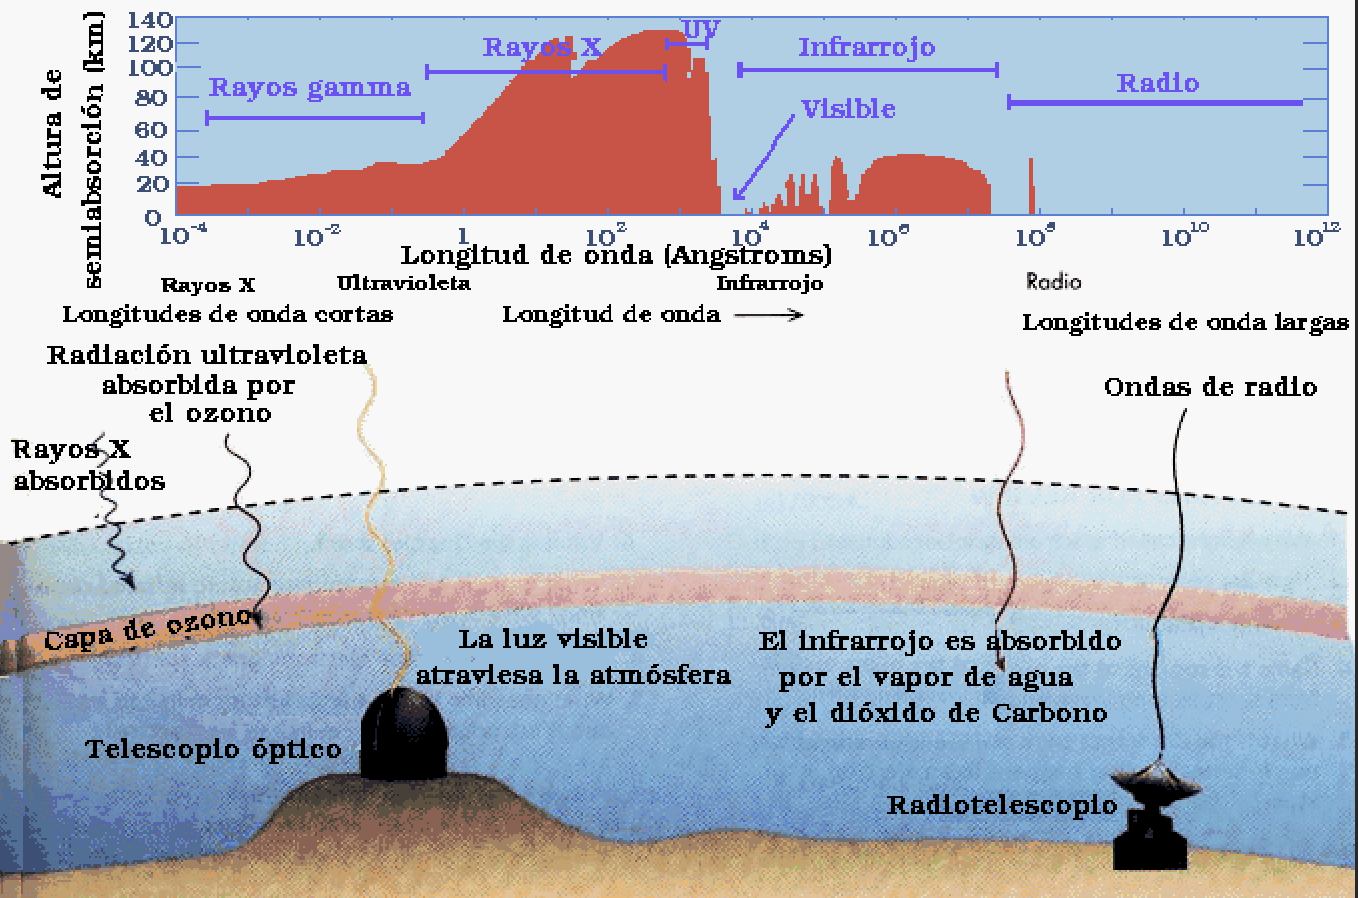
\includegraphics[width=1.0\linewidth]{figura1.png}
        \caption{Ejemplo de figura}
        \label{fig:figura1}
\end{figure}
Para citar una figura en el texto, se utiliza el comando \verb|\ref{}|  Por ejemplo, si queremos referirnos a la Figura~\ref{fig:figura1}, simplemente escribimos \ref{fig:figura1}.

\section{Resultados}

Presentación de los resultados obtenidos.

\section{Discusión}

Discusión de los resultados obtenidos.

\section{Conclusiones}

Conclusiones del artículo.

\section*{Agradecimientos}
En esta parte se pueden incluir agradecimientos a personas, instituciones o proyectos.

\section*{Referencias bibliográficas}
Para incluir la lista de referencias bibliográficas se puede hacer de las dos formas que se indican abajo: ingresando cada referencia con el comando "bibitem" en este documento, o usando un el archivo bibligrafia.bib.
Para citar una referencia bibliográfica en el texto, se utiliza el comando \verb|\cite{}|. Por ejemplo, si queremos citar un artículo de un autor llamado Scargle publicado en 1982, escribimos \cite{scargle_1982}, que se encuentra en este caso en el listado de artículos dentro del archivo bibliografia.bib.

%Forma 1 de incluir referencias
\begin{thebibliography}{}
   \bibitem{smith2005}
    Smith, J. (2005). Título del artículo. Nombre de la revista, vol. 1, páginas 1-10.
    \bibitem{jones2010}
    Jones, A. (2010). Título del libro. Editorial X.
\end{thebibliography}


%Forma 2 de incluir referencias
\bibliography{biblio}


\end{document}